
%(BEGIN_QUESTION)
% Copyright 2011, Tony R. Kuphaldt, released under the Creative Commons Attribution License (v 1.0)
% This means you may do almost anything with this work of mine, so long as you give me proper credit

Identify the three transmitters in this ``three element'' boiler feedwater control system, and also identify what would happen to the boiler water level if the instrument air supply to the feedwater valve failed (i.e. the supply air pressure fell to 0 PSI):

$$\includegraphics[width=15.5cm]{i04407x01.eps}$$

\underbar{file i04407}
%(END_QUESTION)





%(BEGIN_ANSWER)

{\it 2 points for each correct transmitter identification, 4 points for correct consequence of air failure.}

\vskip 10pt

Drum level transmitter = {\bf LT-690}

\vskip 10pt

Steam flow transmitter = {\bf FT-693}

\vskip 10pt

Feedwater flow transmitter = {\bf FT-691}

\vskip 10pt

If instrument air fails, the boiler will {\bf run dry} because FV-691 is fail-closed (FC).

%(END_ANSWER)





%(BEGIN_NOTES)


{\bf This question is intended for exams only and not worksheets!}.

%(END_NOTES)

